\section{Hard X-Ray spectroscopy}

One of the diagnostic systems present in most of the currently existing tokamaks
is the Hard X-Ray Monitor (HXRM). It will also be used in ITER.
The device is tasked with measuring the spectrum of X-Ray radiation
inside the fusion vessel. The presence of high energy X-Ray
radiation can point to problems with the plasma stability and suggest the 
need for mitigation techniques.
\cite{low_noise_amplifier_for_pmt}

\subsection{Runaway electrons}

The plasma in a tokamak is super-heated so that particles reach a velocity
that enables them to break through atomic repulsion. In such conditions some 
particles can also obtain sufficient speed to escape the vessel's magnetic confinement.
Typically collisions with other particles are so frequent
that in stable plasma these effects are rare.
Directly after plasma is disrupted or terminated, 
the probability of collisions is lessened 
and a tokamak might start behaving like a particle accelerator,
accelerating the electrons to nearly the speed of light.
Electrons that act in this manner are called Runaway Electrons (REs).
\cite{iter_re_melt}

This phenomenon can occur in the form of a high-energy 
concentrated beam capable of melting the front-facing walls of a reactor.
The effects of such damage being purposefully introduced in the JET tokamak
are shown in \autoref{fig:re_melt}. To prevent and mitigate the destructive
effects of REs their generation has to be avoided if possible. Otherwise
they must be detected and dealt with. Typically the plasma 
is cooled, or the electromagnets are accentuated
to reduce the disruptions. More extreme methods might 
involve the injection of noble gases in a process called 
Massive Gas Injection (MGI) \cite{massive_gas_injection}.
\begin{figure}[H]
  \centering
  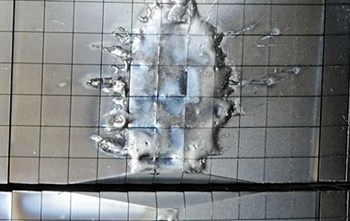
\includegraphics[width=.7\linewidth]{media/re_melt.jpeg}
  \caption{Effects of RE in the JET vessel \cite{iter_re_melt}}
  \label{fig:re_melt}
\end{figure}


When REs interact with the Plasma Facing Components (PFCs)
they lose their energy and emit X-Ray radiation in 
the Bremsstrahlung process. The energy of this radiation
varies greatly, ranging from tens of keV (Soft X-Ray)
to multiple MeV (Hard X-Ray).
\cite{hxrm_jet}

\subsection{PhotoMultiplier Tubes}

The photons generated in Bremsstrahlung by Runaway Electrons
can be detected with the use of a device known as a PhotoMultiplier Tube (PMT).
A PMT is built with the use of a photocathode and an electron multiplier.
When a photon hits the photocathode an electron is emitted
due to the photoelectric effect. The electric fields inside the PMT accelerate the 
electron towards a series of dynodes. Each collision with a dynode releases
additional electrons and forms a stronger beam that 
eventually reaches the anode, where it becomes measurable as a current pulse.
\autoref{fig:pmt} shows the internal structure of a PMT together with the output
signal, a sharp exponentially decaying current pulse.
\cite{pmts_basics, pmt_gain}
\begin{figure}[H]
  \centering
  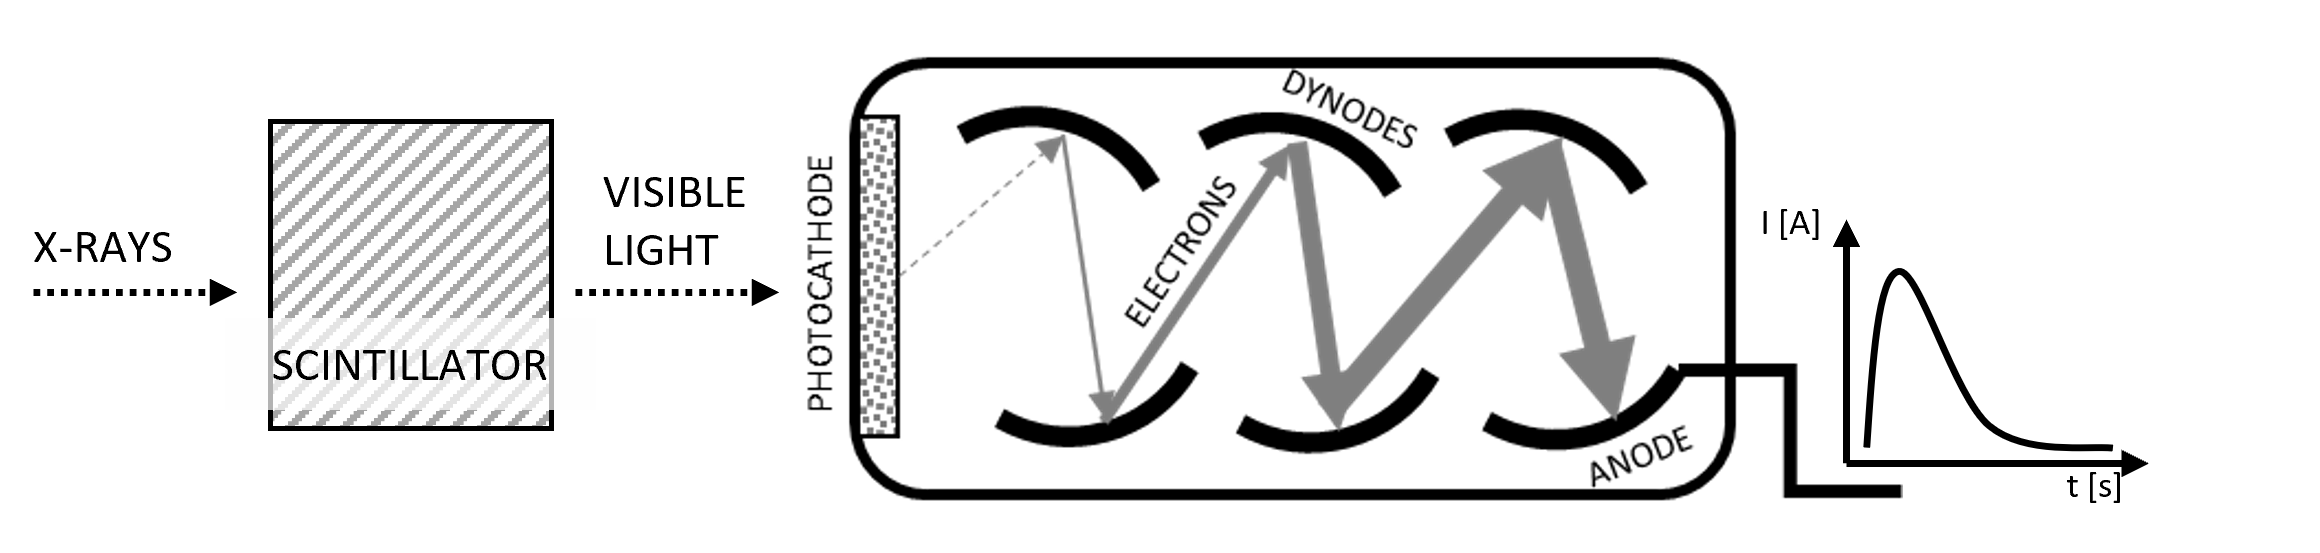
\includegraphics[width=.7\linewidth]{media/pmt.png}
  \caption{A PhotoMultiplier Tube}
  \label{fig:pmt}
\end{figure}
\subsection{Preamplifiers}

The internal gain of a PMT, obtained from the electron multiplication
is sufficient for many applications. The produced current impulses 
can be detected with precise circuitry,
however there are multiple reasons for which
a preamplifier is often used in tangent with a PMT. With a typical
load of $50 \: \Omega$ the output signal of a single photon is
a very sharp voltage peak of around 10 mV.
These short pulses can be detected with precise instruments and used for counting 
and timing purposes, but may be problematic when it comes to discrimination and 
more advanced processing like Pulse Height Analysis (PHA).
\cite{why_pmt_need_amplifiers}


In those scenarios that do not require the sharpest response,
the slight increase in Signal to Noise Ratio (SNR) is worth the 
features introduced by an amplifier. These can include
impedance matching, filtering and pulse-shaping.
In fusion reactors it also helps move most of the 
diagnostic infrastructure away from the difficult environment
created by the fusion plasma. 
Long wiring is susceptible to ElectroMagnetic Interference (EMI), 
so the millivolt signal produced by a PMT would 
get drowned out in the plasma-induced interference without amplification.

\subsection{Pulse processing chains}

To obtain a radiation spectrum from the voltage pulses,
their height must be measured and
placed into an appropriate bin consisting of a range of voltage levels.
The pulses generated by a PMT last just a few nanoseconds,
making the task at hand complicated.
With a preamplifier this duration is increased by a value
that depends on the preamplifier components.
This results in pulses that last a few hundreds nanoseconds.
Before the advent of ultra-high speed Analogue to Digital Converters (ADCs),
such short events could not viably be processed with digital 
electronics and had to rely on analogue components.

\subsubsection{Analogue processing chains}

In analogue radiation spectroscopy
pulses are typically first transformed to a Gaussian shape,
with a series of low- and high-pass filters.
These signals must then pass through complicated pile-up
rejection circuitry. After that the pulses 
are fed to a Multi Channel Analyzer (MCA).
This is the device that performs the binning action.
Initially an MCA would consist of an array of 
analogue comparators, and over time it would rely 
on more and more digital components.
The schematics of a typical analogue system are shown in \autoref{fig:analogue_pp}

\begin{figure}[H]
  \centering
  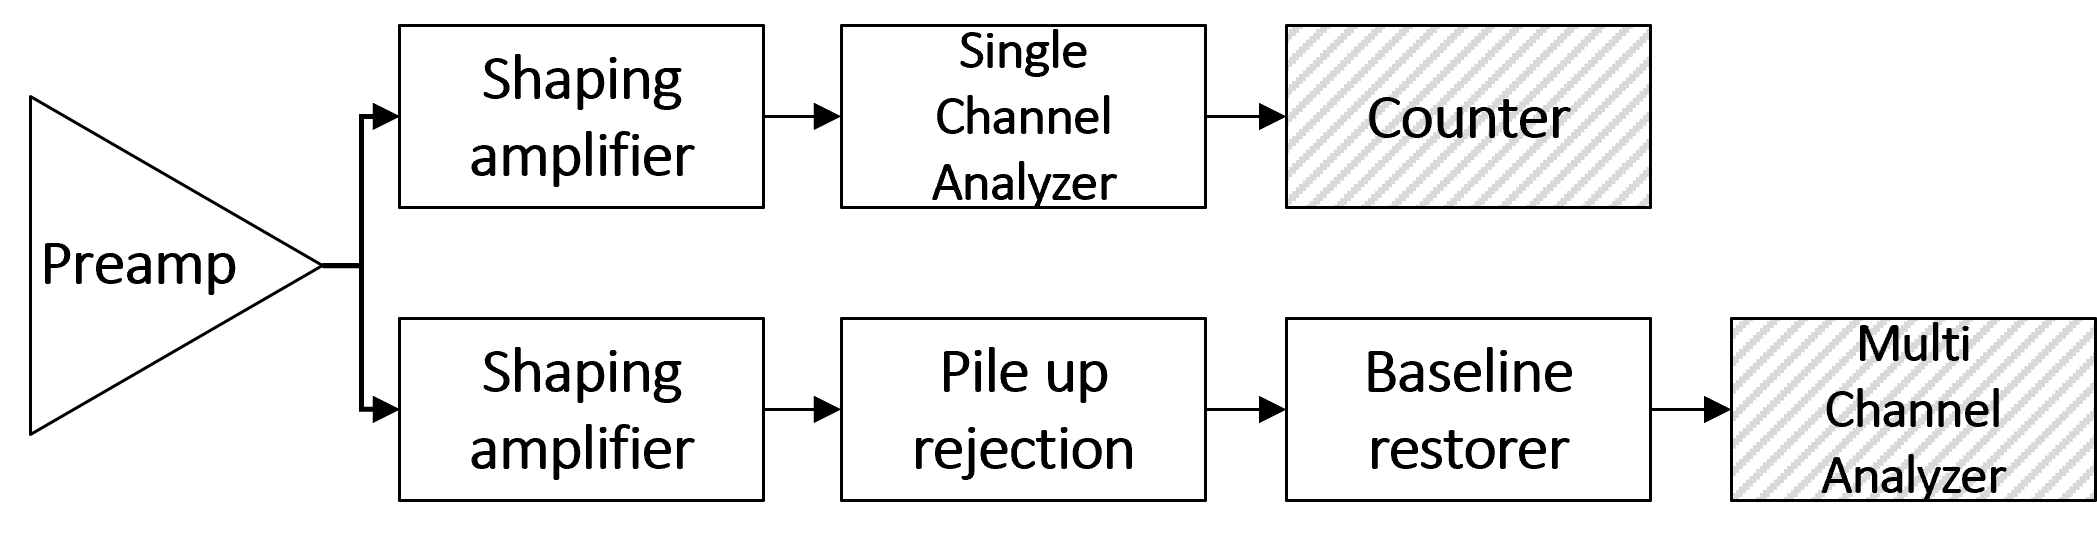
\includegraphics[width=\linewidth]{media/analog_pulse_processing.png}
  \caption{Analogue Pulse Processing chain}
  \label{fig:analogue_pp}
\end{figure}


As mentioned earlier, for a long time analogue processing 
was the only way to reliably handle events shorter than 100 ns. 
It was, however, quickly recognized
that a more digital approach offered 
much lesser susceptibility to outside noise. 
Digital components could also potentially be tuned without
having to physically modify the circuit.
These two features are particularly important in the 
complicated environment of a fusion reactor.
\cite{analog_vs_digital_1998}

\subsubsection{Digital processing chains}

As soon as ADCs and digital processing circuits capable of
reaching the resolution required for precise nuclear
spectroscopy appeared on the market, they were 
adopted into new experimental designs of MCAs \cite{mca_fpga}.
As the technology improved, ADCs were moved closer to the 
radiation detector itself.
A single reprogrammable silicon chip, together with a fast ADC,
could perform the job of multiple analogue components
in a spectroscopy system.
On top of that, its operation is less susceptible to Electro Magnetic
Interference (EMI) and temperature-induced parameter variance.
\cite{dpp_walewski}


The earlier in a processing chain that the ADC is placed the
lesser the influence of the imperfect analogue components is.
An ADC being inserted right after the preamplifier is commonplace
in modern systems as shown in \autoref{fig:digital_pp}.
Such approach, produces an important issue.
To obtain a sufficient horizontal resolution, comparable to analogue systems,
the ADC must sample the signal with a frequency of at least
a few hundred MHz. This means that, at a typical vertical resolution
of anywhere between 8 to 16 bits, a modern high-speed ADC
can generate anywhere between 100 megabytes 
up to even a few gigabytes of data every second.
\cite{dpp_walewski}

\begin{figure}[H]
  \centering
  
\includegraphics[width=.7\linewidth]{media/digital_pulse_processing.png}
  \caption{Digital Pulse Processing chain}
  \label{fig:digital_pp}
\end{figure}

Processing gigabytes of data in real time poses one of 
the primary challenges in designing Digital Pulse Processing systems.
Despite that, fast digitizers are used for Hard X-Ray Spectroscopy
in existing tokamaks, like KSTAR or JET \cite{hxrm_jet, kstar_upgrade}.
ITER will require similar or better systems during its operation,
so the problems of handling large data throughput
should be considered solved before the diagnostic systems
are installed on site. Once first plasma is obtained,
the possibility of hardware modifications will be greatly limited.
 

\subsection{ITER HXRM specification}

The Hard X Ray Monitor planned to be installed at ITER will 
have to meet very specific requirements. The device 
has to operate in two modes. The first mode is the pulse 
counting mode. In it the pulses produced by the PMT have to be
detected, categorized and binned. This actions has to be 
performed continuously over a configurable time period between
1 ms and 10 ms. Each sampling window must then produce an 
energy spectrum of the collected pulses. 
\cite{iter_hxrm_ddd}


Although storing the entire spectrum
is useful for research purposes, two figures must be transferred 
as quickly as possible to the Plasma Control System (PCS), so that
critical decisions regarding the tokamak's safety can be made.
The PCS requires the maximum runaway electron energy measured
and the total count to operate. This data has to be made available
with a latency lesser than 5 ms after each sampling window.
\cite{iter_hxrm_ddd}


When the number of runaway electrons becomes overwhelming for
the PMT detector, the signal produced by the device will 
appear closer to a constant current, due to the pulse overlap.
When that scenario occurs the HXRM must switch into its second 
mode of operation, the current mode. In this mode the PCS 
must be sent the electric current magnitude measured over the 
same time window. It is expected that a switch to current mode
will be made when the number of pulses exceeds $10^6$ counts per second.


On top of the spectral information sent to PCS,
the device should also transfer unprocessed (raw) samples with the detected pulses
to the Data Archiving Network (DAN) for offline analysis and diagnostics.
\autoref{tab:hxrm_specification} lists the most important 
parameters that ITER's HXRM must meet. 
The table includes parameters related to operation 
in both counting and current modes.

\begin{table}[H]
\caption{Selected ITER's requirements for the HXRM \cite{iter_hxrm_ddd}}
\centering
  \begin{tabular}{l | l}
  {\bfseries Parameter} & {\bfseries Value}\\
  \hline
  \textit {RE Energy Range}             & 0.1 MeV to 100 MeV \\ \hline
  \textit {Required energy resolution}  & 20\% \\ \hline
  \textit {RE current to be detected}   & 10 kA to 15 MA\\ \hline
  \textit {ADC sampling period}         & 2 ns\\ \hline
  \textit {Number of ADC channels}      & 2\\ \hline
  \textit {Max. detector temperature}   & 240 \degree C $\pm$ 10 \degree C\\ \hline
  \textit {Max. magnetic field}         & 5 T\\ 
  \end{tabular}
  \label{tab:hxrm_specification}
\end{table}


To meet the requirements regarding temperature and magnetic field,
as well as the space constraints, some important considerations were taken. 
In ITER the X-Ray radiation will first be converted to a light pulse 
with a scintillator.
Only the scintillator will be exposed directly on the front wall.
The PMT detector will be connected to the scintillator via a 12 m long
optical fiber. The PMT will then interface to the processing system through
a 100 m long coaxial cable.
\cite{nowakowski_future_hxrm}


The attentuation of fiber optic is usually specified in 
dB/km so 12 m is a length insufficient to generate meaningful light loss.
The critical issue lies in the connectors. Miscoupling of 
fiber optic connectors can generate a massive signal loss.
In a tokamak's environment it will be nearly impossible to keep the 
connectors perfectly aligned due to vibrations, temperature variation
and magnetic fields. It is thus likely that just a few promilles 
of the photons generated by the scintillator will actually reach 
the PMT. 
\cite{nowakowski_future_hxrm}
